Please note, unit tests were executed using JUnit.  The NLPUtilityTest class
is included here in Section \ref{sec:unittests}.  Please reference the
NLPUtilityTest class for details on what each unit test verifies.
\newline
\begin{wrapfigure}{r}{0.6\textwidth}
	\fbox{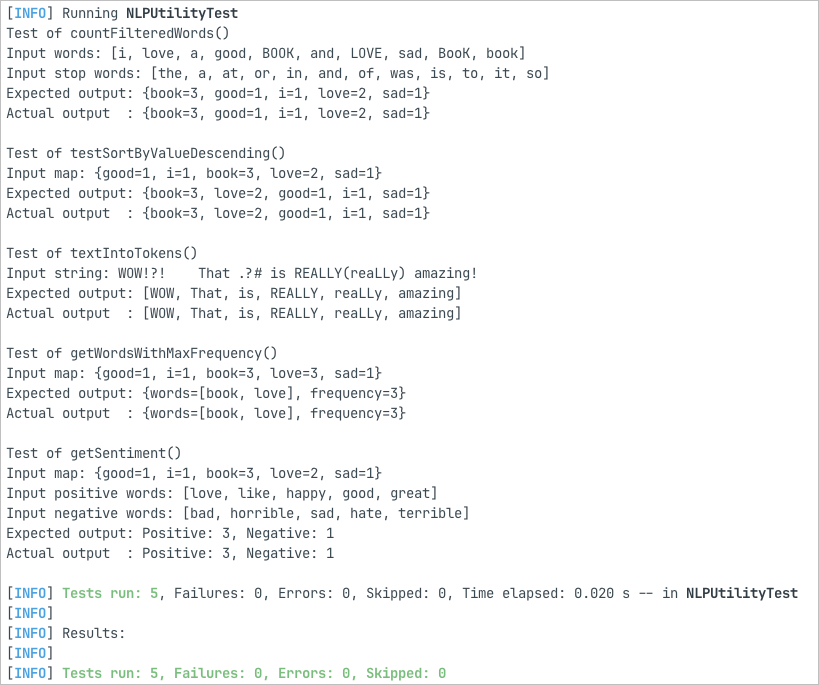
\includegraphics[width=1.0\linewidth]{images/unittests.png}}
	\caption{Unit Tests, via JUnit}
\end{wrapfigure}
Expected output:\newline
\begin{lstlisting}
 Running NLPUtilityTest
 Tests run: 5, Failures: 0, Errors: 0, Skipped: 0, Time elapsed: 0.023 s -- in NLPUtilityTest

 Results:

 Tests run: 5, Failures: 0, Errors: 0, Skipped: 0
\end{lstlisting}
